\documentclass[border=2pt]{standalone}
\usepackage{tikz}
\usetikzlibrary{intersections, arrows.meta, decorations.pathmorphing, backgrounds, fit, positioning, petri}

\begin{document}
    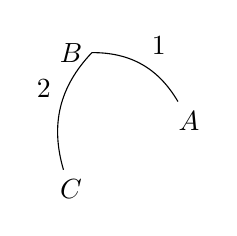
\begin{tikzpicture}[auto, bend right]
        \node (A) at (0:1) {$A$};
        \node (B) at (120:1) {$B$};
        \node (C) at (240:1) {$C$};

        \draw (A) to node[swap] {1} (B) to node[swap] {2} (C);
    \end{tikzpicture}
\end{document}